\section{Arquitectura general del proyecto}
\label{sec:Arquitectura-general}

Antes comenzar a detallar los diferentes sprints donde se explica el desarrollo de cada avance, se presenta la arquitectura final del sistema, para que el lector pueda entender el flujo completo y como fue desarrollandose.

Como se muestra en la Figura~\ref{fig:arquitectura-general}, el sistema se divide en tres bloques principales.


El primero es \textbf{Django}, que actúa como núcleo de la aplicación. Dentro de este bloque, el módulo de ingestión se encarga de validar la URL introducida por el usuario,descargar el contenido de la API de forma segura y detectar automáticamente el formato de los datos, ya sea JSON, XML, CSV o GeoJSON. A continuación, el módulo de análisis LLM procesa la estructura del dataset y propone un schema con los campos más relevantes,que el usuario puede revisar y modificar antes de continuar. Una vez aceptado el plan, el generador produce un proyecto Django completo en siete pasos secuenciales, generando desde los modelos y vistas hasta los templates HTML y los ficheros de infraestructura necesarios para el despliegue. Todo el proceso queda registrado en la base de datos PostgreSQL, que almacena tanto los modelos de la aplicación como los logs de cada llamada al LLM para facilitar la depuración. Finalmente, el módulo de notificaciones informa al usuario en los momentos clave del flujo: al registrarse, al iniciar sesión y cuando su sitio ha sido generado correctamente.

El segundo es \textbf{n8n}, que gestiona las automatizaciones más costosas en tiempo y que no pueden ejecutarse de forma síncrona desde Django. En total se desarrollaron seis workflows, agrupados en dos categorías. Por un lado, los workflows de \textbf{autenticación y notificación}: \textit{Login} y \textit{Register} gestionan el envío de correos al usuario al iniciar sesión o registrarse, y \textit{generation-done}
notifica al usuario cuando su sitio ha sido generado correctamente. Por otro lado, los workflows de \textbf{infraestructura}: \textit{deploy} recibe la señal de Django mediante un webhook, construye la imagen Docker del proyecto generado, arranca el contenedor en un puerto libre y verifica que el sitio ha quedado operativo antes de devolver la URL de preview; \textit{health-check} se ejecuta de forma programada comprobando diariamente que el servidor sigue activo y alertando al administrador si detecta algún problema; y \textit{auto-shutdown} apaga automáticamente los contenedores que llevan inactivos más de un tiempo configurable, liberando recursos del servidor sin intervención manual.

El tercero son los \textbf{servicios externos}, que el sistema consume pero no controla. El proveedor de LLM, ya sea Groq, OpenRouter o un modelo configurado por el propio usuario, recibe los prompts del módulo de análisis y del generador y devuelve las respuestas en texto plano. Las APIs públicas son la fuente de datos que el usuario introduce en el sistema y de las que Django descarga el contenido a procesar. El servidor de correo recibe las notificaciones de n8n y las entrega al usuario final. Por último, el host Docker es el entorno donde se ejecutan los contenedores de los sitios generados, accesibles mediante una URL de preview.

La comunicación entre Django y n8n se realiza exclusivamente mediante webhooks, de forma que ambos sistemas están desacoplados y un fallo en las automatizaciones nunca bloquea el funcionamiento principal de la aplicación.

%%%%%%%%%%%%%%%%%%%%%%%%%%%%%%%%%%%%%%%%%%%%%%%%%% 

\begin{figure}[H]
    \centering
    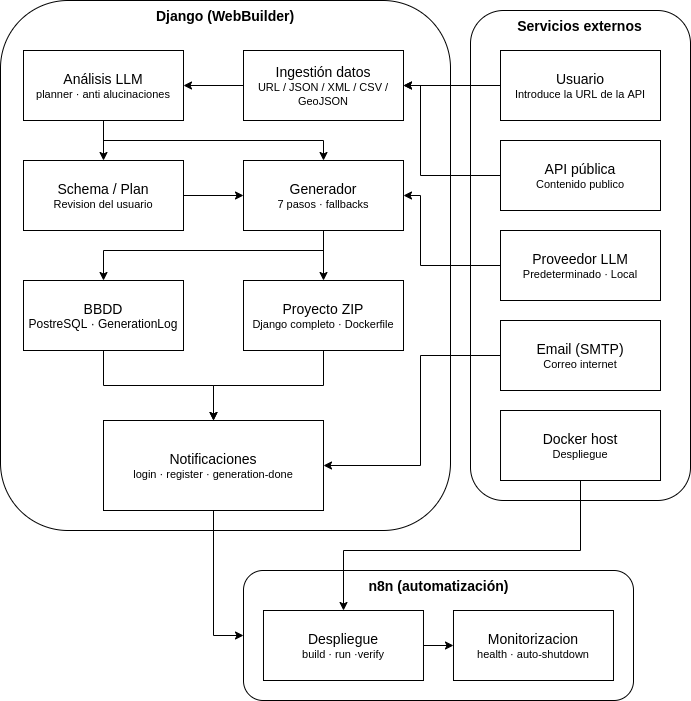
\includegraphics[width=\textwidth]{img/disenoimplementacion/arquitecturageneral}
    \caption{Arquitectura general del sistema WebBuilder}
    \label{fig:arquitectura-general}
\end{figure}